\chapter{Altri argomenti}
\section{Discrete Time Markov Chains}
Una Catena di Markov a Tempo Discreto (DTMC) è una struttura matematica utilizzata per modellare sistemi che evolvono in modo probabilistico, passo dopo passo, in tempi discreti. Formalmente, una DTMC è definita come una tupla $(U,X,Y,p,g)$, in cui:
\begin{enumerate}
    \item \textit{Insieme di input ($U$):} Può essere vuoto, finito o infinito. Rappresenta l'insieme degli ingressi che influenzano il sistema. 
    \item \textit{Insieme di stati ($X$):} Deve essere non vuoto e rappresenta tutte le configurazioni possibili del sistema.
    \item \textit{Insieme di output ($Y$):} Deve anch'esso essere non vuoto e rappresenta i valori osservabili che il sistema può generare.
    \item \textit{Funzione di probabilità di transizione ($p$):} È una funzione $p:X\times X\to[0,1]$ che restituisce la probabilità che il sistema passi da uno stato $x\in X$ a uno stato $x'\in X'$ dato un input $u\in U$, ovvero $p(x'|x, u)$. La somma delle probabilità per ogni stato successivo deve essere pari a 1, ovvero $\int_{X'}p(x'|x,u)dx'=1$.
    \item \textit{Funzione di output ($g$):} È una funzione $g:X\to Y$ che associa ogni stato del sistema $x\in X$ a un valore di output $y\in Y$.
\end{enumerate}
Per semplicità di notazione, si usa indicare i componenti con $M(U)$, $M(X)$, $M(Y)$ per riferirsi rispettivamente agli input, stati e output di una DTMC.

\subsection{Esempi di utilizzo delle DTMC}
\begin{Example}{Tempo di completamento}{}
\textit{Consideriamo un processo software che attraversa tre fasi: definizione dei requisiti, sviluppo del sistema e test del sistema. Ogni fase ha una durata media e delle probabilità di transizione tra stati:}

\begin{minipage}{\textwidth}
    \centering
    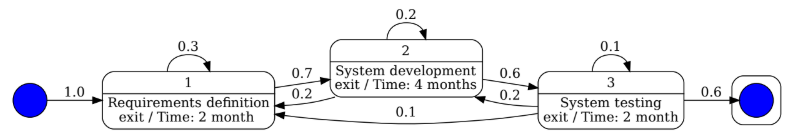
\includegraphics[width=0.9\textwidth]{images/es1-dtmc.PNG}
    %\captionof{figure}{}
\end{minipage}

\begin{itemize}
    \item \textit{Definizione dei requisiti:} La fase iniziale ha una durata di 2 mesi. Se il processo non termina, ci sono due possibilità per proseguire: può andare direttamente alla fase di sviluppo o ripetere la fase di definizione dei requisiti. La probabilità di avanzare alla fase successiva è  0.7 e la probabilità di restare in questa fase è 0.3.
    \item \textit{Sviluppo del sistema:} Questa fase ha una durata di 4 mesi. Le probabilità di avanzare o restare sono rispettivamente  0.6 e 0.2. Se il processo non termina in questa fase, può tornare alla fase precedente con probabilità 0.2.
    \item \textit{Test del sistema:} Infine, il test del sistema ha una durata di 2 mesi. Le probabilità di passare alla fase finale, ovvero l'uscita, è 0.6. Se il processo non termina in questa fase, può tornare alle fasi precedenti o rimanere nella stessa fase con probabilità 0.2, 0.1 e 0.1.
\end{itemize}
L'obiettivo è calcolare la probabilità che il processo termini esattamente in 8 mesi. Il percorso possibile è: $0\to 1\to 2\to 3\to 4$. La probabilità totale si ottiene moltiplicando le probabilità lungo questo percorso:
\begin{equation*}
    1.0\times 0.7\times 0.6\times 0.6=0.252
\end{equation*}

Considerando lo stesso processo software, immaginiamo ora di voler calcolare la probabilità che termini in esattamente 10 mesi. Per calcolare questa probabilità, dobbiamo considerare i percorsi possibili che portano a una durata totale di 10 mesi. I percorsi sono:
\begin{gather*}
Percorso 1: 0\to 1\to 1\to 2\to 3\to 4\\
Percorso 2: 0\to 1\to 2\to 3\to 3\to 4
\end{gather*}
La probabilità per ciascun percorso viene calcolata moltiplicando le probabilità di transizione lungo il percorso:
\begin{align*}
    1.0 \times 0.3 \times 0.7 \times 0.6 \times 0.6 +\\ 1.0 \times 0.7 \times 0.6 \times 0.1 \times 0.6 =\\ 0.07560 + 0.02520 =\\ 0.1008
\end{align*}
Quindi, la probabilità che il processo termini esattamente in 10 mesi è 0.1008.

Immaginiamo ora di voler calcolare la probabilità che il processo software descritto in precedenza termini in esattamente 12 mesi. Come nel caso precedente, dobbiamo considerare tutti i percorsi che portano a una durata totale di 12 mesi.
\begin{align*}
Percorso 1: & 0\to 1\to 1\to 1\to 2\to 3\to 4\\
Percorso 2: & 0\to 1\to 1\to 2\to 3\to 3\to 4\\
Percorso 3: & 0\to 1\to 2\to 2\to 3\to 4\\
Percorso 4: & 0\to 1\to 2\to 3\to 3\to 3\to 4    
\end{align*}

Le probabilità totale viene calcolata come segue:
\begin{align*}
    1.0 \times 0.3 \times 0.3 \times 0.7 \times 0.6 \times 0.6 +\\ 1.0 \times 0.3 \times 0.7 \times 0.6 \times 0.1 \times 0.6 +\\ 1.0 \times 0.7 \times 0.2 \times 0.6 \times 0.6 + 
    \\1.0 \times 0.7 \times 0.6 \times 0.1 \times 0.1 \times 0.6 =\\ 0.022680 + 0.007560 \times 0.05040 \times 0.002520 =\\ 0.08316
\end{align*}
Pertanto, la probabilità che il processo termini esattamente in 12 mesi è 0.08316.
\end{Example}

\begin{Example}{Costo di completamento}{}
\textit{In questo esempio consideriamo un processo software composto da tre fasi principali, ciascuna caratterizzata da un costo fisso e probabilità di transizione che determinano il percorso del sistema.}

\begin{minipage}{\textwidth}
    \centering
    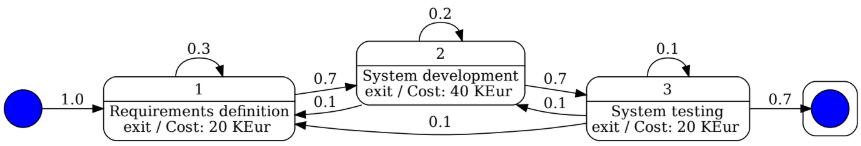
\includegraphics[width=0.9\textwidth]{images/es2-dtmc.PNG}
    %\captionof{figure}{}
\end{minipage}

\begin{itemize}
    \item \textit{Definizione dei requisiti:} La fase iniziale prevede un costo di 20.000 euro ed è obbligatoria. La probabilità di passare alla fase successiva è 0.7, mentre quella di rimanere nella stessa fase è 0.3.
    \item \textit{Sviluppo del sistema:} Questa fase ha un costo di 40.000 euro. La probabilità di avanzare alla fase successiva è 0.7, mentre la probabilità di restare nella fase corrente o tornare indietro è rispettivamente 0.2 e 0.1.
    \item \textit{Test del sistema:} L'ultima fase prima della conclusione prevede un costo di 20.000 euro. La probabilità di completare il processo, ovvero passare alla fase finale di uscita, è 0.7. Altre probabilità includono restare nella fase o tornare indietro (con probabilità 0.1).
\end{itemize}
Supponiamo di voler calcolare la probabilità che il costo totale del processo sia esattamente 80k. Il percorso che soddisfa questa condizione è: $0\to 1\to 2\to 3\to 4$

La probabilità totale di completare il processo seguendo il percorso specificato si ottiene moltiplicando le probabilità delle transizioni lungo il percorso:
\begin{equation*}
    1.0\times 0.7\times 0.7\times 0.7=0.343
\end{equation*}
La probabilità che il processo termini con un costo complessivo di 80.000 è pari a 0.343.
\end{Example}

\begin{Example}{Progettazione}{}
\textit{Consideriamo un processo software che si sviluppa in tre fasi principali. Il sistema è caratterizzato da probabilità di transizione definite, con un parametro variabile $p$ che influenza il comportamento del processo.}

\begin{minipage}{\textwidth}
    \centering
    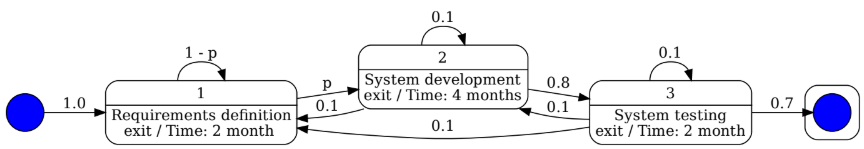
\includegraphics[width=0.9\textwidth]{images/es3-dtmc.PNG}
    %\captionof{figure}{}
\end{minipage}

\begin{itemize}
    \item \textit{Definizione dei requisiti:} La fase iniziale ha una durata di 2 mesi. La probabilità di avanzare o restare nella fase corrente dipende dai parametri forniti, $p$ e $1-p$.
    \item \textit{Sviluppo del sistema:} Questa fase ha una durata di 4 mesi. La probabilità di avanzare, restare nella fase corrente o tornare alla fase precedente sono rispettivamente 0.8, 0.1 e 0.1.
    \item \textit{Test del sistema:} Ha una durata di 2 mesi. La probabilità di completare il processo è pari a 0.7.
\end{itemize}
L'obiettivo è determinare il valore minimo di $p$ che garantisce che il processo termini esattamente in 8 mesi con una probabilità di almeno 0.5.

Il percorso che consente al processo di terminare esattamente in 8 mesi è $0\to 1\to 2\to 3\to 4$. Questo significa che il processo avanza senza ripetere alcuna fase.

La probabilità associata a questo percorso è data dalla moltiplicazione delle probabilità delle transizioni lungo il percorso:
\begin{align*}
    1.0\times p\times 0.8\times 0.7\geq0.5\\p\geq\frac{0.5}{0.8\times 0.7}=\\0.8928
\end{align*}
Il valore minimo di $p$ necessario per garantire che il processo termini esattamente in 8 mesi con una probabilità di almeno 0.5 è 0.8928.

Ora consideriamo lo stesso processo, ma il nostro obiettivo è garantire che il costo totale del processo sia esattamente 80k con una probabilità di almeno 0.5. Anche in questo caso, il valore $p$ influenza le probabilità di transizione.

Il percorso che consente di ottenere un costo totale di 80k è $0\to 1\to 2\to 3\to 4$.

La probabilità associata a questo percorso è:
\begin{align*}
    1.0\times p\times 0.7\times 0.7\geq 0.5\\p\geq\frac{0.5}{0.7\times 0.7}=\\1.02...
\end{align*}
Non esiste un valore di $p$ compreso tra 0 e 1 che soddisfi questa condizione, poiché il valore calcolato è maggiore di 1. Pertanto, non è possibile raggiungere una probabilità di almeno 0.5 che il costo totale del processo sia esattamente 80k.
\end{Example}

\subsection{Reti di DTMC}
Le DTMC possono essere combinate in una rete, in cui ciascun componente è una DTMC autonoma ma interconnessa con le altre. 

\begin{figure}[ht]
    \centering
    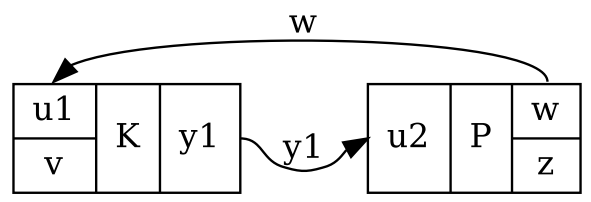
\includegraphics[width=0.35\linewidth]{images/network-dtmc.PNG}
    \caption{Una rete di DTMC}
    \label{fig:network-dtmc}
\end{figure}

Ad esempio, considerando le due DTMC $K$ e $P$ con rispettivamente input $u1$ e $v$ e $u2$ e output $y1$ e $w$ e $z$ (Figura \ref{fig:network-dtmc}). Le DTMC sono collegate tra loro attraverso gli output di una che diventano input dell'altra, in particolare l'output $y1$ di $K$ diventa l'input $u2$ di $P$ e l'output $w$ di $P$ diventa l'input $u1$ di $K$. 

La rete risultante può essere definita come una nuova DTMC, con stati, probabilità di transizione e funzioni di output derivati dai componenti originali. Nel caso precedente la DTMC $M$ risultante avrà input $v$ e output $z$.

Formalmente, siano $K = (U_1\times V, X_1, Y_1, p_1, g_1)$ e $P = (U_2, X_2, W\times Z, p_2, g_2)$ con $K(U_1) = P(W)$ e $P(U_2) = K(Y_1)$ allora
\begin{equation*}
    M = (V, X_1 \times X_2, Z, p, g)    
\end{equation*}
dove
\begin{align*}
    &p((x'_1, x'_2)|(x_1, x_2), v) = p_1(x'_1|x_1,(g_{2,W}(x_2), v))\times p_2(x'_2|x_2, g_1(x_1))\\
    &g(x_1, x_2) = g_{2,Z}(x_2)
\end{align*}
